% Asset ID: FA22FurtherKinematicsTikZ-003
% Source: CCEA FA22-FKIN-LO001
% Related lesson section: Core Theory; Visual Asset Integration
% Used placeholder:
% [VISUAL PLACEHOLDER: FA22FurtherKinematicsTikZ-003 | Source: CCEA FA22-FKIN-LO001 | Insert from tikz/FA22FurtherKinematicsTikZ-003.tex | Purpose: Show 3D position, velocity and acceleration vectors using \(\mathbf{i}\), \(\mathbf{j}\), and \(\mathbf{k}\).]
% Purpose:
% Show 3D kinematics with position vector r(t), velocity vector v(t),
% acceleration vector a(t), and i, j, k unit directions.

\documentclass[tikz,border=8pt]{standalone}

\usepackage{amsmath}
\usepackage{amssymb}
\usetikzlibrary{arrows.meta, calc, positioning}

\definecolor{Canvas}{HTML}{FAF9F6}
\definecolor{Panel}{HTML}{FFFFF0}
\definecolor{Line}{HTML}{E5E5EA}
\definecolor{Text}{HTML}{2C2C2E}
\definecolor{Gold}{HTML}{C5A059}
\definecolor{Rose}{HTML}{FBEFEF}
\definecolor{SoftGold}{HTML}{F6E8B1}

\begin{document}

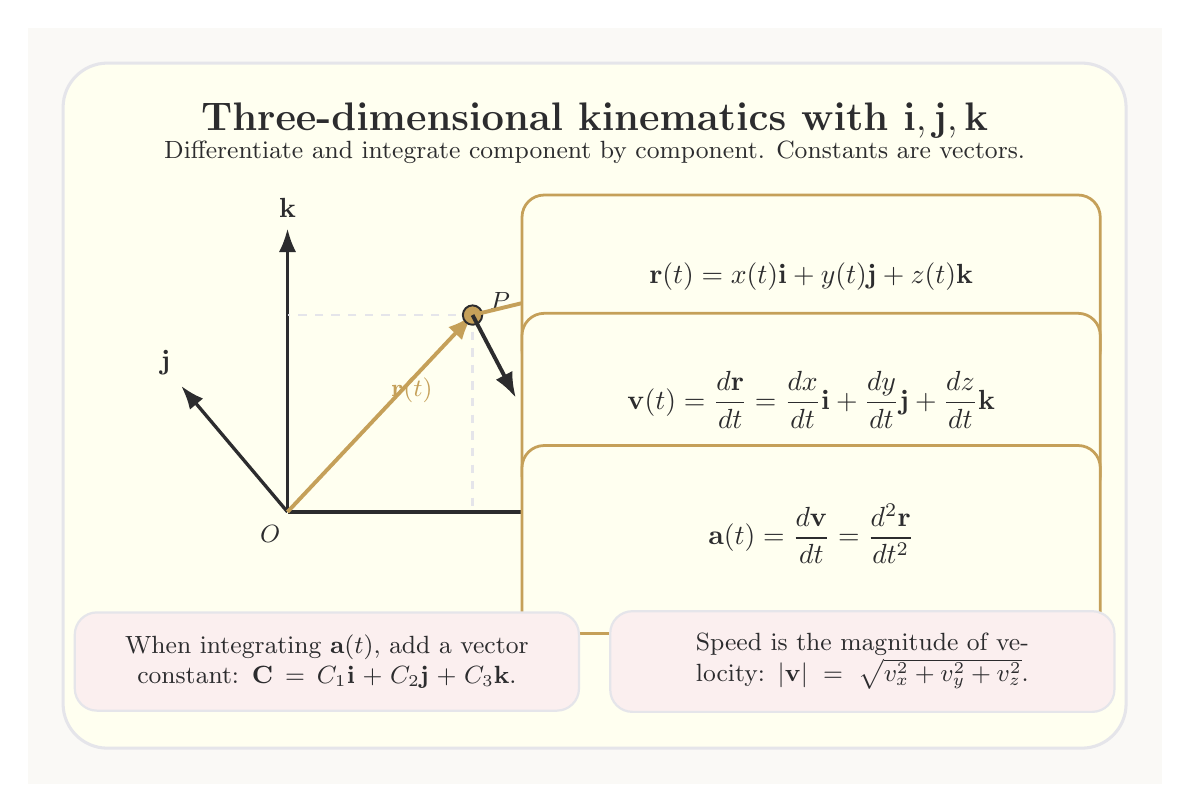
\begin{tikzpicture}[
  font=\sffamily,
  axis/.style={
    -{Latex[length=3mm,width=2.2mm]},
    line width=1.2pt,
    draw=Text
  },
  vector/.style={
    -{Latex[length=3.2mm,width=2.4mm]},
    line width=1.4pt,
    draw=Gold
  },
  accel/.style={
    -{Latex[length=3.2mm,width=2.4mm]},
    line width=1.4pt,
    draw=Text
  },
  note/.style={
    rounded corners=8pt,
    draw=Line,
    line width=0.8pt,
    fill=Rose,
    align=center,
    text=Text,
    inner xsep=10pt,
    inner ysep=8pt,
    font=\small
  },
  formula/.style={
    rounded corners=8pt,
    draw=Gold,
    line width=1.0pt,
    fill=Panel,
    align=center,
    text=Text,
    inner xsep=12pt,
    inner ysep=10pt,
    font=\normalsize
  }
]

\fill[Canvas] (-7.2,-4.8) rectangle (7.2,4.8);
\draw[Line, line width=1.1pt, rounded corners=16pt, fill=Panel]
  (-6.75,-4.35) rectangle (6.75,4.35);

\node[text=Text, font=\bfseries\Large, align=center] at (0,3.62)
  {Three-dimensional kinematics with \(\mathbf{i},\mathbf{j},\mathbf{k}\)};
\node[text=Text, font=\small, align=center] at (0,3.22)
  {Differentiate and integrate component by component. Constants are vectors.};

\coordinate (O) at (-3.9,-1.35);
\coordinate (X) at (-0.35,-1.35);
\coordinate (Y) at (-5.25,0.25);
\coordinate (Z) at (-3.9,2.25);
\coordinate (P) at (-1.55,1.15);

\draw[axis] (O) -- (X) node[below right, text=Text] {\(\mathbf{i}\)};
\draw[axis] (O) -- (Y) node[above left, text=Text] {\(\mathbf{j}\)};
\draw[axis] (O) -- (Z) node[above, text=Text] {\(\mathbf{k}\)};

\node[text=Text, font=\small] at ($(O)+(-0.22,-0.28)$) {\(O\)};

\draw[Line, line width=0.8pt, dashed] (P) -- (-1.55,-1.35);
\draw[Line, line width=0.8pt, dashed] (P) -- (-3.9,1.15);

\draw[vector] (O) -- (P) node[midway, above right, text=Gold, font=\small]
  {\(\mathbf{r}(t)\)};

\fill[Gold] (P) circle (3.5pt);
\draw[Text, line width=0.7pt] (P) circle (3.5pt);
\node[text=Text, font=\small] at ($(P)+(0.35,0.18)$) {\(P\)};

\draw[vector] (P) -- ($(P)+(1.45,0.35)$)
  node[right, text=Gold, font=\small] {\(\mathbf{v}(t)\)};

\draw[accel] (P) -- ($(P)+(0.55,-1.05)$)
  node[below right, text=Text, font=\small] {\(\mathbf{a}(t)\)};

\node[formula, text width=6.5cm] at (2.75,1.55)
  {\[
    \mathbf{r}(t)
    =
    x(t)\mathbf{i}
    +
    y(t)\mathbf{j}
    +
    z(t)\mathbf{k}
  \]};

\node[formula, text width=6.5cm] at (2.75,0.0)
  {\[
    \mathbf{v}(t)
    =
    \frac{d\mathbf{r}}{dt}
    =
    \frac{dx}{dt}\mathbf{i}
    +
    \frac{dy}{dt}\mathbf{j}
    +
    \frac{dz}{dt}\mathbf{k}
  \]};

\node[formula, text width=6.5cm] at (2.75,-1.7)
  {\[
    \mathbf{a}(t)
    =
    \frac{d\mathbf{v}}{dt}
    =
    \frac{d^2\mathbf{r}}{dt^2}
  \]};

\node[note, text width=5.7cm] at (-3.4,-3.25)
  {When integrating \(\mathbf{a}(t)\), add a vector constant:
  \(\mathbf{C}=C_1\mathbf{i}+C_2\mathbf{j}+C_3\mathbf{k}\).};

\node[note, text width=5.7cm] at (3.4,-3.25)
  {Speed is the magnitude of velocity:
  \(\left|\mathbf{v}\right|=\sqrt{v_x^2+v_y^2+v_z^2}\).};

\end{tikzpicture}

\end{document}
